\section{Background} \label{sec:requirements}

This chapter reviews the research and systems the project builds on. It begins with learning analytics and the dashboards that present it, then examines how student behaviour is modelled, how data-driven methods personalise support, and how retrieval-augmented generation grounds language-model feedback; it closes by surveying existing systems, identifying the gaps this thesis addresses, and specifying the requirements that follow from them.

\subsection{Learning Analytics and Dashboards}

This section introduces learning analytics and the dashboards through which it reaches educators: its use in higher education, the role of dashboards as the primary means of presenting it, and the move towards real-time analysis that makes in-session support possible.

\subsubsection{Learning Analytics in Higher Education}



In 2012, the use of data analytics was shown to improve student success by providing real-time feedback, demonstrating the impact of data informed intervention in higher education \cite{nguyen_2020_data,hattiePowerFeedback2007,blackAssessmentClassroomLearning1998}.
Learning analytics is the measurement, collection, analysis, and reporting of data about learners and their contexts in order to understand and optimise learning and the environment in which it occurs \cite{wikipediacontributors_2019_learning_analytics,nguyen_2020_data,siemensLearningAnalyticsEmergence2013,clowOverviewLearningAnalytics2013}. 
The growth of online education since the 1990s has contributed significantly to the advancement of learning analytics, as student data can now be captured and analysed enabling educators to make more data-driven decisions \cite{nguyen_2020_data,vieira_2018_visual,romeroEducationalDataMining2020}. 

Learning analytics draws on a range of data sources: Vieira et al. survey Massive Open Online Courses (MOOCs), clickstream records of interactions such as clicks and time spent, and course content \cite{vieira_2018_visual}. They find that, although combining data types is argued to serve learning outcomes more effectively, the majority of studies still rely on a single source \cite{vieira_2018_visual}. This work does not address live computer-lab sessions; the source that matters for this case is neither retrospective clickstream nor demographic or gaze data, but the stream of code submissions a student produces while working, which this project takes as its primary signal.

The outputs of learning analytics have proven valuable for pedagogical decision-making, from tailoring recommendations to students' behavioural profiles \cite{vieira_2018_visual} to confirming, in the VITAL project, that flipped-classroom delivery worked because students engaged with materials before face-to-face sessions \cite{gelan_2018_affordances}. Wilson et al. caution, however, that such systems read observable behaviours such as clicks and time online rather than the cognitive processes beneath them \cite{wilson_2017_learning}, and that moving analytics beyond the controlled setting raises privacy concerns \cite{wilson_2017_learning,tzimas_2021_ethical}. 
This project addresses the first limitation directly by inferring struggle from submissions as the session goes on, when an instructor can intervene, and respects the second by operating only on session submission data without demographic or biometric profiling so that students cannot be identified.

With the current utilisation of learning analytics, there is a lack of approaches that leverages smart devices in computer labs, in particular, smart watches and smart glasses.
By leveraging smart devices, we can significantly increase the efficiency of lab assistance. 
From a centralised point, we can allow the lab teacher to send instructions to lab assistants based on these analytics, such as which questions are hardest and which students need the most help, thereby improving learning outcomes \cite{vieira_2018_visual,wilson_2017_learning,tzimas_2021_ethical}.

\subsubsection{Dashboards for Learning Analytics}

Learning analytics have been leveraged to use dashboards as valuable tools for both educators and learners, such as making educators aware of subtle interactions in their courses and allowing learners to gain insight into their learning actions and the effects they may have \cite{klerkx_2017_learning,verbert_2013_learning}. Because of capabilities such as these, dashboards are the primary representation of learning analytics, as they can help improve learning outcomes and make the most of the data generated by learning analytics \cite{klerkx_2017_learning,verbert_2013_learning}.

SAM was an early dashboard developed on data from learning environments, with both teachers and learners as target user groups \cite{govaerts_the}. SAM allowed teachers to separate students who were doing well from those at risk based on time spent and resource-use metrics. Teachers gain insight into the time learners spent on tasks and can compare with their estimates, whilst resource use provides insights on how and how often students used documents and tools, it also allows discovery of resources external to the course \cite{govaerts_the}. Metrics could also be added, depending on data detail, to increase understanding of specific tasks \cite{govaerts_the}. EMODA is a more recent approach to the learning dashboard; it takes into account emotion, which researchers have shown to play a key role in learning, regulation processes, and strong coupling to motivation and achievement \cite{verbert_2013_learning}. EMODA enables teachers to monitor learners' emotions during online learning sessions by analysing audio, video, self-reports, and interaction traces \cite{verbert_2013_learning}.

Edsight is a web-based learning analytics dashboard developed with responsive web design that accommodates different device types and is accessible to educators \cite{ahn_2019_the}. When first logging in, teachers are presented with all the practical measure data they have collected thus far, the classrooms with the most data, and how many days have elapsed since they last logged data for analysis \cite{ahn_2019_the}.

\begin{figure}[h]
    \centering
    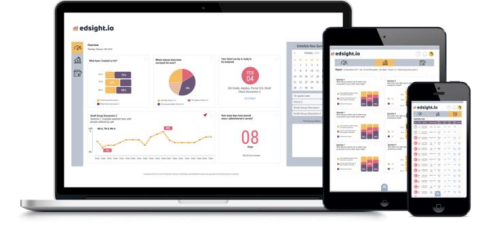
\includegraphics[width=1\linewidth]{figures/requirements-specification/Edsight-Dashboard-1.png}
    \caption{“Overview,” “Report,” and “Activity List” modes, displayed in desktop, tablet, and phone screens.}
    \label{fig: Edsight Dashboard 1}
\end{figure}

The report is the main dashboard in Edsight, where teachers can select filters such as date and classroom for display. Once a filter is applied, different results are displayed.


\begin{figure}[H]
    \centering
    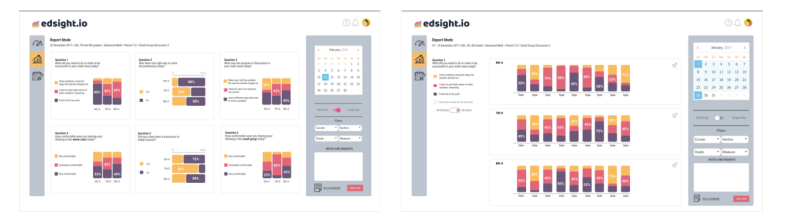
\includegraphics[width=1\linewidth]{figures/requirements-specification/Edsight-Dashboard-2.png}
    \caption{Edsight: (L) a single-event report with filters; (R) the multi-day comparison view.}
    \label{fig: Edsight Dashboard 2}
\end{figure}

Most current approaches to the learning dashboard do not live in lab sessions, as there is more course-level monitoring than session-level monitoring \cite{klerkx_2017_learning,verbert_2013_learning,ahn_2019_the}. This also has many benefits, helping students on the spot and allowing them to get the most out of their computer labs \cite{ahn_2019_the}.

\subsubsection{Real-Time Data Analytics and Visualisation}

Real-time analytics refers to the practice of collecting and analysing data as it is generated, with minimal latency between data collection and analysis \cite{marr_2021_what}. When we can process data as it comes in, we can gain insight and understand what is happening within a relevant context almost instantly. Such a practice is used in applications where data timeliness is critical, such as smart pricing and predictive maintenance \cite{marr_2021_what}. Traditional data analysis, where data is captured and stored, and insights are pushed out of storage. In contrast, real-time data analysis allows data to be analysed in real time. Real-time data analytics have proven to be highly valuable, as evidenced by the success of Netflix, which has perfected the art of predicting its customers' next favourite show \cite{marr_2021_what}.

Real-time analytics has emerged as a pivotal tool across multiple sectors, including retail, revolutionising decision-making processes and operational strategies \cite{mustafaayobamiraji_2024_realtime}. Retail giants such as Walmart and Amazon have leveraged real-time data analytics to personalise marketing campaigns, optimise pricing strategy, and efficiently manage inventory \cite{mustafaayobamiraji_2024_realtime}. Technologies such as RFID, IoT, and advanced analytics platforms were used to gather real-time data, analyse customer behaviour, and make data-driven decisions \cite{mustafaayobamiraji_2024_realtime}. A less utilised but more relevant application is in education, for example, a real-time machine learning application that detects learners' attention levels and participation using sensory data. The data allows teachers to recalibrate their teaching as necessary \cite{montebello_assisting}.

\begin{figure}[H]
    \centering
    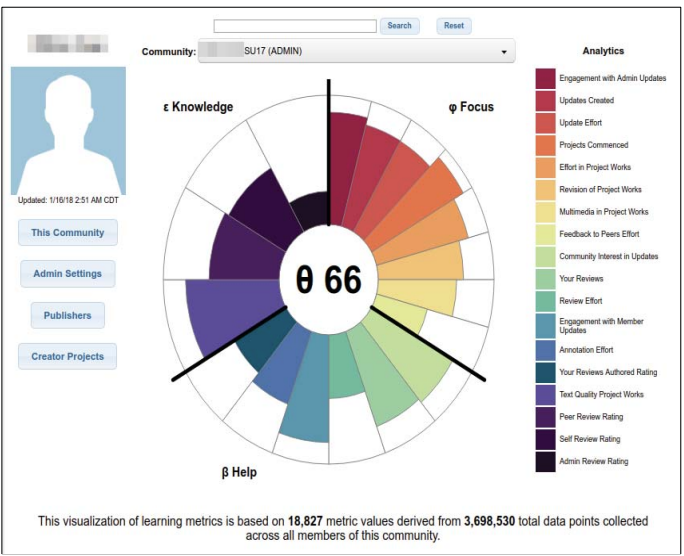
\includegraphics[width=1\linewidth]{figures/requirements-specification/Attention-Dashboard.png}
    \caption{The Learning Analytics Interface for a dashboard which collects data based on student attention}
    \label{fig: Attention Dashboard}
\end{figure}

Applying real-time analytics in computer labs will prove to be very beneficial for students and teachers alike. By collecting and processing data as it comes in, we will be able to update dashboards in real time and provide teachers with the most up-to-date information, enabling relevant, timely support. This would be better than a traditional data analysis approach, in which we review the data after the lab has finished, because our findings may not be relevant by then \cite{montebello_assisting,mustafaayobamiraji_2024_realtime}.

\subsection{Modelling Student Behaviour}

This section reviews how observable lab behaviour is modelled. 
It covers four themes in this area: detecting student struggle in the moment, tracing the growth of skill mastery over time, estimating which questions are hardest for the class, and training the composite signals that combine these. 
Student struggle and question difficulty are treated as complementary targets throughout: one identifies who needs help, the other identifies what the class as a whole finds hardest.


\subsubsection{Modelling Student Struggle}
A key challenge in supporting students during lab sessions is identifying which students are struggling and may require timely intervention. 
Studies in education have approached struggle detection at different temporal scales, ranging from within-assignment detection to course-level.
Dong et al.\ highlighted an approach that detects moments of struggle during a session based on time spent and progress relative to peers, achieving over 77\% accuracy when validated against expert judgement on whether intervention was needed \cite{dong_using}.
Struggle has been operationalised as failing the same unit test consecutively for more than four submission events, providing a clear threshold-based criterion \cite{dong_using}.

Beyond threshold-based approaches, more sophisticated methods have been explored. 
In related work, Or examined novice programmers' testing behaviour as an early step toward defining coding struggle, identifying patterns such as repeatedly submitting the incorrect answer for more than four submission events, signalling that students have stopped making meaningful progress \cite{or_2024_exploring,beckWheelSpinningStudentsWho2013}.
To move this even further, Estey et al.\ proposed a trajectory metric that measures changes in programming behaviour over time across a four-semester study of 514 students \cite{estey_2017_automatically}. 
Their early predictor identified 81\% of students who struggled throughout the course, but also flagged 43\% who went on to succeed, highlighting the difficulty of distinguishing slight from serious struggle.
Their trajectory metric reduced this false-positive rate to 11\%, demonstrating the importance of tracking how performance changes rather than measuring the students' current level \cite{estey_2017_automatically}.

Another approach uses machine learning to build a graphical model of how students navigate through programming assignments. By capturing the full solution trajectory, Piech et al.\ showed that a student's progression path is predictive of later difficulty, motivating the inclusion of the student's trajectory to track changes in answer quality across submissions \cite{piech_modeling}.

A complementary approach is knowledge tracing which models how a student's mastery of underlying skills progresses over time and it is examined in the next subsection.

Recent work on Large Language Models (LLMs) is also relevant as AI-generated feedback can provide more valuable insights than raw correctness alone.
Koutcheme et al.\ show that language models LLMs that are better at helping repair student programs also provide better explanations of coding issues, suggesting that the quality of LLM feedback can be studied empirically rather than assumed \cite{koutcheme_using}
More broadly, Pitts et al.\ survey LLM-based applications in programming education and argue that these systems are most effective when combined with human oversight rather than fully autonomous replacements \cite{pitts_a}

Together, these works demonstrate different methods for evaluating struggle. These metrics are best captured through a combination of temporal, correctness-based and behavioural signals.

\subsubsection{Knowledge Tracing and Bayesian Student Models}
A related but distinct line of work is knowledge tracing, which models how a student's mastery of underlying skills progresses over time.
Bayesian Knowledge Tracing (BKT) remains attractive because it is interpretable and computationally manageable.
Khajah shows that BKT can gain a performance boost by merging it with Item Response Theory (IRT) to model multidimensional problem difficulties and student abilities, without fitting student specific parameters, allowing the model to be generalisable to new students \cite{khajah_supercharging}.
In programming education, Kim et al.\ propose a knowledge tracing approach that integrates students' questions and automatically extracted skill information, showing that textual interaction data can provide useful signals about understanding misconception patterns \cite{kim_knowledge}.
This is relevant to the current project, as it suggests that struggles during computer labs should not be treated solely as repeated failures but also as informed by temporal behaviour, how the student develops, and question-specific context.  

Bayesian Knowledge Tracing was formalised by Corbett and Anderson in the context of an intelligent programming tutor, which treats the student's knowledge of each skill as either in a learned state or an unlearned state that can transition from unlearned to learned based on the student's interactions \cite{corbettKnowledgeTracingModeling1995}.
The model is governed by four interpretable parameters: an initial-learning probability, $p(L_0)$, an acquisition probability, $p(T)$ that a skill transitions from unlearned to learned at each practice opportunity, a guess probability, $p(G)$ for correct responses without mastery and a slip probability, $p(S)$ for incorrect responses despite mastery. The probability of a correct response on the next opportunity is then 
\begin{equation}
    p(C) = p(L) \cdot (1 - p(S)) + (1 - p(L)) \cdot p(G),
    \label{eq:bkt-prediction}
\end{equation} 
where $p(L)$ is the current estimate of mastery \cite{corbettKnowledgeTracingModeling1995}.
Here $p(L_0)$ is the prior probability of mastery before any attempt, whereas $p(L)$ is the running estimate after each observed response, updated by Bayes' rule and advanced by the transition $p(T)$; the full update is given in Section~\ref{sec: bkt}.
The original formulation assumes no forgetting, so the latent state cannot transition from learned back to unlearned.

Yudelson et al.\ extended BKT by individualising parameters across students and showed across KDD datasets that this yielded tangible improvements when predicting unseen student data \cite{yudelsonIndividualizedBayesianKnowledge2013}. They found that individualising the speed of learning $p(T)$ produced consistent gains in predictive accuracy, while individualising the prior $p(L_0)$ alone had no measurable effect, suggesting learning rate is the more important axis of student variation for BKT to exploit.

More recent work has explored neural alternatives to BKT such as deep learning approaches. Piech et al.\ proposed Deep Knowledge Tracing (DKT),  with two different types of Recurrent Neural Networks (RNNs): a Long Short Term Memory (LSTM) based model and a vanilla RNN model with sigmoid unit. These models predict a student's future performance based on their past activity. This resulted in a 25\% gain in the area under the curve (AUC) over the best previous result on a knowledge tracing benchmark as well as showing that knowledge tracing models do not need expert annotations \cite{piechDeepKnowledgeTracing2015}.
However, Khajah et al.\ subsequently showed that BKT extended with forgetting, latent student abilities, and automatic skill discovery matches DKT performance on average across four different data sets, arguing that the gains of deep approaches stem from added flexibility rather than from any representation discovery \cite{khajahHowDeepKnowledge2016}.
For an instructor facing dashboard, where the interpretability of mastery estimates is essential, BKT remains a defensible choice.

\subsubsection{Modelling Task Difficulty}


Alongside students' struggles, it is important to identify which questions pose the greatest difficulty for the class as a whole so that teachers can address the problem in front of the whole class rather than just for the student.
Dannath et al. examined task-level struggle detection methods in intelligent tutoring systems for programming, noting that prior work focused on dropout prevention rather than understanding the student's path towards the correct solution for a specific task \cite{dannath_evaluating}.
The separation in modelling is important as students may appear to be struggling with a genuinely difficult question rather than with individual performance. 
Additionally, if most of the class is struggling with a problem, it will be faster to go through the question with the whole class.

Task difficulty can be inferred from indicators such as failure rate, average time spent, number of attempts and the amount of feedback used before reaching a correct answer \cite{dannath_evaluating,piech_modeling}.
These measures are useful as they are directly observable and can be updated during a live session with low cost, but they do not separate question difficulty from variation in student ability.

Alternatively, we can model difficulty using Item Response Theory (IRT), which offers a more principled approach by accounting for how difficult a question actually is, rather than raw counts, as well as a student's latent ability \cite{rasch1960probabilistic,lord1968statistical}. It is worth noting that IRT captures how difficult a question is from the way students respond to it, which is not always the same as how hard the question is to learn or teach.
Baucks et al.\ uses IRT to analyse course difficulty variation and show how applying latent variable models can uncover meaning patterns in course rigor that is hidden when relying on simple metrics \cite{frederikbaucks_2024_gaining}. 
In online learning environments that allow multiple attempts, Pankiewicz argues that measuring task difficulty becomes more complex because task difficulty and feedback shape how it should be interpreted, motivating methods that go beyond raw metrics. \cite{pankiewicz_measuring}  
These works support the view that question difficulty should be modelled separately from student struggle and, where possible, that composite measures should be used rather than a single measure.

Overall, the literature suggests that task difficulty should be deduced from a combination of correctness, time, attempts, and progression-related information rather than from a single descriptive statistic \cite{dannath_evaluating,piech_modeling}.


\subsubsection{Composite Model Training and Optimisation}

Supervised learning allows us to refine composite weights through methods such as ordinary least squares (OLS) regression \cite{hastieElementsStatisticalLearning2009} or gradient boosting against externally-collected labels.
This method serves as an alternative to hand-set or manually tuned weights.
The supervised approach does not need to be human annotated as we can now leverage LLMs as raters; recent studies demonstrate substantial agreement with human annotators on classification tasks at a small cost and saving time \cite{gilardiChatGPTOutperformsCrowd2023, chiangCanLargeLanguage2023, zhengJudgingLLMasaJudgeMTBench2023, liuGEvalNLGEvaluation2023}.
Rather than tuning hyperparameters manually we can use modern Bayesian optimisation libraries such as Optuna's Tree-structured Parzen Estimator (TPE) to efficiently search the hyperparameter space and tune the scalar hyperparameters that govern these composite models \cite{NIPS2011_86e8f7ab, akibaOptunaNextgenerationHyperparameter2019}, as TPE produces stable optima in fewer iterations than other methods such as grid search and random search.

\subsection{Data-Driven Personalisation}

This section examines two data-driven techniques that move beyond scoring each student in isolation. 
Collaborative filtering infers a student's likely need for help from peers with similar interaction profiles, while text mining recovers the common mistake patterns hidden in free-text answers across the cohort. 
The two are complementary: one personalises at the level of the individual learner, the other surfaces structure shared across the class.



\subsubsection{Collaborative Filtering}

Beyond parametric approaches discussed in the previous subsection, more sophisticated data-driven methods have been explored in the educational recommender systems literature \cite{dasilva_2022_a, deschnes_2020_recommender}.
Collaborative filtering is an alternative method used for personalising user experiences \cite{resnickGroupLensOpenArchitecture1994}.
Unlike methods that rely on parameters, Collaborative filtering leverages the collective behaviour of users with similar histories to create preferences, on the principle that users with similar histories share similar needs \cite{schafer_2007_collaborative}. This method has been applied primarily in educational contexts to provide more efficient and accurate course suggestions than traditional methods \cite{li_2020_course}. This can be done with different types of models, such as linear regression and factor decomposers. It is evident that integrating intelligent recommendation technology significantly enhances resource utilisation and the overall student learning experience

A user-based collaborative filtering method identifies a set of $k$ nearest neighbours for a given student based on a similarity measure over their profiles \cite{herlockerAlgorithmicFrameworkPerforming1999}. The behaviour of the neighbours are aggregated to produce a prediction. The approach is shown to be effective in sparse datasets, where explicit ratings are unavailable and implicit signals such as time-on-task and submission frequency must serve as proxies for preference. A known limitation is that when a student has little interaction history, similarity cannot be computed reliably, leading to unstable early-session predictions.

In the context of lab struggle detection, collaborative filtering offers a strong alternative to our scoring approach. Rather than computing a fixed weighted score for each student, it can identify students whose interaction patterns closely resemble peers who need help, inferring that they too may need help. However applying collaborative filtering to a live computer lab comes with its constraints as students who may need help is limited and the start of the session will have very limited data. These constraints backs the use of a scoring approach, whilst the collaborative filtering approach is a strong alternative.


\subsubsection{Text Mining and Mistake Pattern Recovery} \label{sec: text mining}

Where student responses are free-text rather than numerical or categorical,
 identifying common mistake patterns requires text-mining techniques that combine information retrieval and unsupervised clustering.
Salton et al.\ introduced the vector space model for information retrieval, which represents documents and queries as vectors in a vector space, allowing for the computation of similarity between them \cite{saltonVectorSpaceModel1975}.
The standard weighting scheme is term frequency-inverse document frequency (TF-IDF) formalised in modern information retrieval as
\begin{equation}
    \mathrm{tf-idf}_{t, d} = \mathrm{tf}_{t, d} \cdot \log\frac{N}{\mathrm{df}_t},
    \label{eq:tfidf}
\end{equation}
where $\mathrm{tf}_{t, d}$ is the frequency of term $t$ in document $d$, $N$ is the total number of documents, and $\mathrm{df}_t$ is the number of documents containing term $t$ \cite{manningIntroductionInformationRetrieval2006}.

Once each document is represented as a TF-IDF vector, similar documents can be partitioned into clusters that share characteristic content.
MacQueen's $k$-means algorithm partitions $n$ points into $k$ clusters to minimise within cluster variance
\cite{MacQueen1967SomeMF}. 
Formally, this corresponds to choosing $k$ centres $C$ that minimise the sum of squared distances from each point to its closest centre,
\begin{equation}
    \phi = \sum_{x \in X} \min_{c \in C} \|x - c\|^2,
    \label{eq:kmeans}
\end{equation}
where $X$ is the set of data points \cite{arthurKmeansAdvantagesCareful}.
Because this objective is non-convex and sensitive to initialisation, Arthur and Vassilvitskii's $k$-means++ seeds initial centres by selecting each new centre with probability proportional to its squared distance from the nearest already-chosen centre, yielding provable approximation guarantees and faster convergence in practice \cite{arthurKmeansAdvantagesCareful}.

Choosing the number of clusters $k$ is itself a problem. Rousseeuw's silhouette coefficient quantifies how well each point fits its assigned cluster relative to the next-nearest cluster:
\begin{equation}
    s(i) = \frac{b(i) - a(i)}{\max\{a(i), b(i)\}},
    \label{eq:silhouette}
\end{equation}
where $a(i)$ is the mean intra-cluster distance for point $i$ and $b(i)$ is the mean distance from $i$ to all points in the nearest other cluster, with values close to $+1$ indicating tight well separated clusters \cite{rousseeuwSilhouettesGraphicalAid1987}. 
Sweeping $k$ and selecting the value that maximises the mean silhouette gives a principled auto-selection rule.
Once clusters are formed, a large language model can produce natural-language cluster explanations \cite{wangGoalDrivenExplainableClustering2023}.

\subsection{Retrieval-Augmented Feedback}
This section reviews the techniques that allow LLM feedback to be trusted in an educational setting. 
The central concern is hallucination: a model that generates fluent but unverified text can mislead a student who cannot yet judge its correctness. 
Retrieval-augmented generation addresses this by grounding the model's output in retrieved source material, and the subsections that follow cover both the generation step, the dense-embedding and approximate-nearest-neighbour retrieval that supplies it.




\subsubsection{Retrieval-Augmented Generation}

Lewis et al.\ introduced Retrieval-Augmented Generation (RAG) as a way to combine parametric language models with a non-parametric retriever over an external source, allowing the generator to condition its output on relevant evidence retrieved at query time \cite{lewisRetrievalAugmentedGenerationKnowledgeIntensive2020}.
 Additionally, RAG models hallucinate less and generate factually more correct text than BART \cite{lewisRetrievalAugmentedGenerationKnowledgeIntensive2020}.
Lewis et al.\ showed that RAG outperformed parametric models on knowledge intensive tasks, including open-domain QA tasks  \cite{lewisRetrievalAugmentedGenerationKnowledgeIntensive2020}.

In educational contexts, the case for retrieval is even stronger. 
Kasneci et al.\ survey the opportunities and challenges of large language models in education, noting that there is a difficulty in distinguishing between real knowledge and convincingly written but unverified model output due to the ability of LLMs to generate human-like text which can make it difficult for students to distinguish between real knowledge and unverified model output leading students to accept false or misleading information as true. 
To mitigate this risk, it is recommended we provide education on how information can be evaluated critically and teach students exploration, investigation, verification and corroboration strategies \cite{kasneciChatGPTGoodOpportunities2023}.
Retrieval-augmented generation can help mitigate this risk by grounding the model's output in verifiable sources, allowing students to trace the information back to its origin and evaluate its credibility \cite{lewisRetrievalAugmentedGenerationKnowledgeIntensive2020,kasneciChatGPTGoodOpportunities2023}.

\subsubsection{Dense Retrieval and Approximate Nearest Neighbour Search}

Before the retrieval step in RAG, we need a representation that captures semantic similarity between documents and queries.
Reimers and Gurevych proposed Sentence-BERT (SBERT), which is a modification of pre-trained BERT that uses siamese and triplet network structures to derive semantically meaningful sentence embeddings that can be compared using cosine similarity \cite{reimersSentenceBERTSentenceEmbeddings2019}.
In the paper they show that commonly used approaches to derive sentence embeddings from BERT such as CLS-token outputs or averaging the BERT output embeddings perform worse than averaged GloVe embeddings on standard semantic textual similarity benchmarks. Siamese fine-tuning on natural language inference data substantially improves correlation on STS benchmarks and outperforms sentence-embedding methods such as InferSent and Universal Sentence Encoder \cite{reimersSentenceBERTSentenceEmbeddings2019}.

Once documents are embedded, exact nearest neighbour search scales linearly with the number of documents which is unfeasible for large retrieval over large collections.
To relax this, Approximate Nearest Neighbours Search (K-ANNS) was proposed, which relaxes the condition of the exact search by allowing a small number of errors in exchange for faster than linear time complexity \cite{malkovEfficientRobustApproximate2016}.
Malkov and Yashunin proposed Hierarchical Navigable Small World (HNSW) graphs, which are a fully graph based ANN index that incrementally builds a multi-layer structure of proximity graphs for nested subsets of the stored elements \cite{malkovEfficientRobustApproximate2016}.
As queries descend greedily from top to the zero layer, logarithmic complexity is achieved, with the evaluation showing that HNSW outperforms previous open source vector only approaches \cite{malkovEfficientRobustApproximate2016}.

Together retrieval-augmented generation, dense sentence embeddings, and approximate nearest neighbour search build the standard pipeline for grounding LLM output.

\subsection{Existing Systems}

This section surveys systems already deployed in education to locate where the present work sits. 
It reviews learning management systems, instructor-facing dashboards, early-warning systems for at-risk students, and the recent class of real-time classroom support systems that sits closest to this work. 
The first three operate largely at the level of the course and review data after the fact; the last bring analytics into the live session, and it is against these that the present contribution must be positioned.

\subsubsection{Learning Management System }
A learning management system administers, tracks and delivers educational courses and materials \cite{wikipediacontributors_2019_learning_management_systems}; such systems hold the largest share of the learning-systems market, almost every higher-education institution has adopted one, and Moodle is the most widely used \cite{wikipediacontributors_2019_learning_management_systems}. They were designed to surface learning gaps through analytics but that reporting has two properties to address: it is reviewed after an activity has finished, so a student who struggled in a lab may already have left without timely help, and it is utilised at the level of the course. Course-level reporting is well suited to curriculum design and long-term planning but it is not suited to the live lab, where support is only useful before the student moves on. It is precisely this gap that the present work targets.

\subsubsection{Instructor Facing Dashboards}

Learning management systems often incorporate dashboards that visualise student progress so that teachers can locate knowledge gaps \cite{kiatxin_development}; the dashboard has become the central output of learning analytics. Existing examples such as Blocks: Progress Bar report active time, assignment progress, marks and submission counts \cite{kiatxin_development,holsteinIntelligentTutorsTeachers2017a,holsteinStudentLearningBenefits2018}. What they report, however, is how far a student has progressed, not whether a student is struggling, and they do so at the course level rather than the live session. This project keeps the dashboard format but pivots it from progress tracking towards real-time struggle and difficulty within the session itself.


\begin{figure}[H]
    \centering
    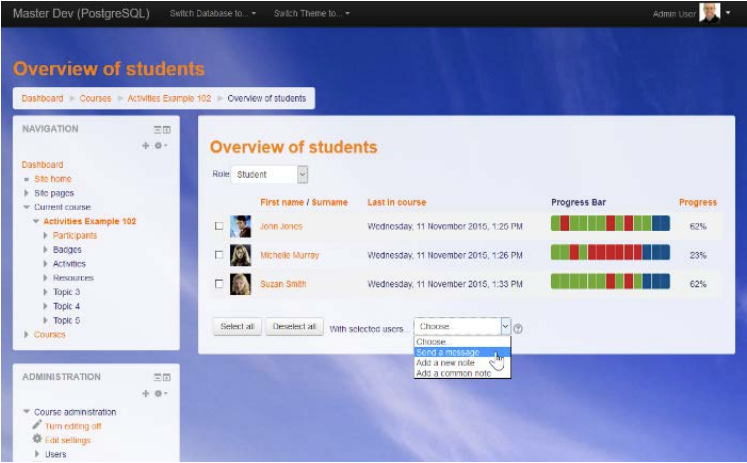
\includegraphics[width=1\linewidth]{figures/requirements-specification/Piwik-Analytics.png}
    \caption{Piwik Analytics}
    \label{fig: Piwik Analytics}
\end{figure}

Another implementation of a learning dashboard is the Multi-Modal (MM) teacher dashboard, the MM dashboard: 1) receives data from eye trackers, wristbands, web cameras, and the learning activity; 2) computes the student’s relevant cognitive, affective, and physiological measurements; 3) synchronises and visualises the resulting measurements in a clean, customisable interface; and 4) notifies instructors during potential moments of interest \cite{leecultura_2023_multimodal}.
\begin{figure}[H]
    \centering/u
    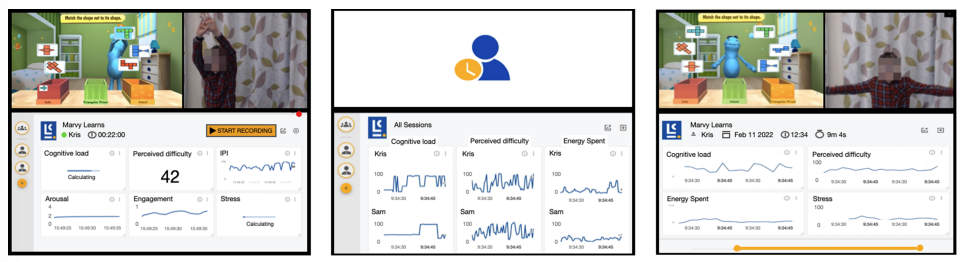
\includegraphics[width=1\linewidth]{figures/requirements-specification/MM-Dashboard.png}
    \caption{Different views of MM dashboard: SSV (left), ASV (centre), and RSV (right).}
    \label{fig: MM dashboard}
\end{figure}
The MM dashboard has three ways of data visualisation, as we can see in \ref{fig: MM dashboard}: 1) single session view (SSV), which displays real-time learning data from a single student’s session; 2) all sessions view (ASV), which shows real-time learning data from all connected students; and 3) replay session view (RSV), which allows the teacher to interact with previously recorded session data from a single student session \cite{leecultura_2023_multimodal}. The views are divided into panels, and we can also see that the SSV and ASV have a right-side navbar used to switch between panels \cite{leecultura_2023_multimodal}.

However, the dashboards do come with a range of issues. For the MM dashboard to work, students must have a range of sensors, which are uncommon for them \cite{leecultura_2023_multimodal}. Teachers also report no experience with some of the hardware required for the MM dashboard to work. Although this is a key problem, it was not the MM dashboard's main issue; the main issue was that teachers may lack the knowledge to understand and interpret the dashboard results, as the majority of users reported unfamiliarity with the measurements provided. The importance of the metrics was also questioned \cite{leecultura_2023_multimodal}. The study also noted that hands-on training may be required to help teachers use the system efficiently \cite{leecultura_2023_multimodal}.

The limitations highlight a critical gap in the practicality and potential for utilisation of the learning dashboards. Whilst the dashboards provide high-level insights, many of these insights are difficult to understand, prompting educators to question their importance. Also, these dashboards tend to be unintuitive, which can be especially an issue for educators who are not STEM-oriented. We can leverage these insights to create clearer indicators, such as struggle, and by taking a more straightforward approach to the dashboard, we can address these gaps and create better, more useful learning dashboards.


\subsubsection{Early Warning and At-Risk Student Systems}

Early warning systems in education identify students at risk of poor learning outcomes by analysing routinely collected data and surface those students to instructors before failure becomes irreversible \cite{macfadyenMiningLMSData2010}.
In education, an At-risk student system is an early warning system that spots struggling students before it is too late \cite{baeres_2020_an}. 
Recently, many approaches to at-risk student systems have leveraged AI to identify students at risk \cite{baeres_2020_an}.


Student data is analysed to flag potential issues. Typically, grades, attendance, online activity, and behaviour are used to alert teachers to help students early, before problems grow \cite{baeres_2020_an}. The datafication of education enables the use of automated methods to detect patterns in extensive educational data. Approaches leverage predictive models to use the data, predicting the likelihood that a student will fail a course \cite{baeres_2020_an}.

We can look at the edInsight Early Warning System as an example. This system looks at the course as a whole and uses the information gained to determine an at-risk ranking for all students \cite{a2020_atrisk}. The system leverages a scoring system, based on specific categories such as the Course grade category \cite{a2020_atrisk}:

\begin{table}[H]
    \centering
    \begin{tabular}{|c|c|}
        \hline
        Grade & Score\\
        \hline
        \hline
        C- & 2 \\
        \hline
        D+ & 4\\
        \hline
        D & 8\\
        \hline
        F & 10\\
        \hline
    \end{tabular}
    \caption{Grade-based scoring: lower grades raise the struggle score.}
    \label{tab: grade scoring}
\end{table}
With the scores calculated, educators have a clear idea of which students are most at risk, making this information useful for directing attention to those who need the most help \cite{a2020_atrisk}.
The same approach has been validated in academic environments. Arnold and Pistilli describe the Course Signals system at Purdue, which is an early intervention system that combines grade, past academic history and demographic predictors into a traffic light indicator for instructors, reporting measurable gains in student retention \cite{arnoldCourseSignalsPurdue2012a}.
Jayaprakash et al.\ generalises this further with an open-source initiative, the Open Academic Analytics Initiative (OAAI), which has been deployed across multiple US institutions, demonstrating that the underlying predictive techniques are not specific to a single platform \cite{jayaprakashEarlyAlertAcademically2014}.


Although the system is beneficial for identifying students who are struggling at the course level, it does not necessarily help identify students at the lab level, as its design assumptions do not align with the demands of lab sessions. Educators working in real-time sessions require live data. Hence, they have immediate awareness of which students are currently struggling, rather than future failure. However, we can apply the same concepts used in at-risk systems to identify students who are struggling the most and questions that have the most difficulty. As a result, as a result while traditional at risk systems are not designed for lab sessions, the underlying principles can be adapted to meet the needs of real-time lab analytics.


\subsubsection{Real-Time Classroom Support Systems}

The closest prior work brings analytics into the live programming session itself. Diana et al.\ present an instructor dashboard that predicts, from live program-state logs, which students need help during an interactive programming assignment \cite{dianaInstructorDashboardRealtime2017}; the same group separately matches low-performing students to higher-performing peer tutors. 
ClassAid moves into orchestration: it places a configurable tutoring agent alongside each student and gives the instructor a live dashboard to monitor the student-AI interaction and switch each agent between technical, heuristic, automatic and silent feedback modes \cite{zhangClassAidRealtimeInstructorAIStudent2026}. Both keep an instructor in the loop, yet neither derives a per-submission correctness signal, ranks question difficulty separately, or clusters the cohort's mistakes.

A related line of work delivers awareness through specialised hardware. 
Lumilo, a set of mixed-reality glasses, presents per-student detector states and Bayesian mastery estimates to a teacher, directing attention to the students who need it most without interrupting the class \cite{holsteinIntelligentTutorsTeachers2017a, holsteinStudentLearningBenefits2018}. The multi-modal teacher dashboard described pursues the same goal through eye-trackers, wristbands and cameras \cite{leecultura_2023_multimodal}. These systems show that real-time awareness is valuable, but they are dependent on the use of certain hardware which may be inaccessible and some stop at awareness rather than routing a person to the student.

A meta-analysis of classroom orchestration systems finds that teacher awareness is the function most strongly associated with improved outcomes, yet awareness on its own does not direct help to where it is needed \cite{fengEffectivenessFunctionsClassroom2023}. Each system above provides one or two of the capabilities this project brings together, but none unites an automatically-derived per-submission correctness signal, separate rankings of student struggle and question difficulty, live clustering of cohort mistakes, and the dispatch of a human assistant over a mobile channel. Table~\ref{tab:rt-systems} summarises how these systems compare with the current project.

\begin{table}[H]
\centering
\small
\setlength{\tabcolsep}{4pt}
\begin{tabular}{|l|c|l|c|c|l|l|}
\hline
System (year) & Live & Signal source & Strug. & Diff. & Dispatch & Device \\
\hline\hline
\textbf{This work} & Y & logs + LLM correctness & Y & Y & human assistant & mobile \\
\hline
Diana (2017) & Y & program-state logs & Y & N & peer (separate) & desktop \\
\hline
ClassAid (2026) & Y & LLM + interaction & part. & N & AI agent & desktop \\
\hline
Lumilo (2018) & Y & ITS detectors + BKT & part. & N & awareness & MR glasses \\
\hline
MM dashboard (2023) & Y & physiological sensors & part. & N & awareness & desktop \\
\hline
\end{tabular}
\caption{Real-time classroom support systems compared with the developed system in this report}
\label{tab:rt-systems}
\end{table}


\subsection{Research Gaps}

This subsection reviewed a range of relevant literature. Learning analytics has proved incredibly useful in higher education by providing data on MOOC completion rates, click counts, and time spent, which have significantly aided pedagogical decision-making. Learning dashboards have also emerged as the primary output of learning analytics, enabling educators to gain insight into how different students are performing through an intuitive user interface. Real-time analytics has enabled processing data as it arrives, benefiting multiple sectors. 
The review also examined the methods that can turn this data into actionable signals: struggle detection, knowledge tracing and Bayesian student models, item-response and composite approaches to question difficulty, collaborative filtering, text mining for mistake-pattern recovery, and retrieval-augmented generation for grounded feedback. 
Each of these have been well established on their own, the gap this thesis addresses lie at their intersection, in the setting of a live computer lab session. 
While the systems reviewed above show that real-time dashboards and classroom orchestration tools exist, a systematic review finds that learning analytics dashboards have not reliably improved student achievement \cite{kaliisaHaveLearningAnalytics2024}; the contribution therefore lies not in another visualisation, but in integrating these signals and acting on them within the session.

In particular, computer labs face a distinct challenge that existing approaches don't address well. In these settings, teachers and assistants have no way to swiftly identify those who need help and must rely on those who put their hands up. The problem with this is that it does not account for shy students who may not want to put their hands up, causing them to spend too much time on a question. Also, current dashboards focus on data collected towards the end of the lab; this data may not be as valid afterwards. 
A dashboard built on real-time analytics addresses this issue directly by leveraging the data as it is generated to support students during the session itself, rather than after it, when intervention is no longer possible.

Three gaps emerge from the work on signals and detection. 
First, LLMs have been studied as a source of explanatory feedback \cite{koutcheme_using, pitts_a} and, in orchestration systems, as tutoring agents dispatched to the student \cite{zhangClassAidRealtimeInstructorAIStudent2026}, but not as a live correctness signal which combines metrics such as correctness, attempt amount and time into a struggle score. 
Where LLMs have instead been asked to judge difficulty directly they align poorly with human-perceived difficulty \cite{liCanLLMsEstimate2025, tabibTrustworthyDifficultyAssessments2025}, which motivates combining the model's signal with item-response and Bayesian estimates rather than relying on it alone.
Second, struggle detection operates largely at the course level \cite{estey_2017_automatically}, and where it is applied within a session it rests on simple threshold rules, such as four consecutive failed submissions \cite{dong_using}, which capture only one of the several factors, time, attempts, trajectory and answer quality, that signal difficulty. 
Third, collaborative filtering is well established for course recommendation \cite{li_2020_course, schafer_2007_collaborative}, yet its use for real-time lab struggle detection is unaddressed, in part because the sparsity of data at the start of a session makes similarity hard to compute reliably \cite{herlockerAlgorithmicFrameworkPerforming1999}.

Two further gaps address understanding the cohort as a whole. Bayesian Knowledge Tracing has been used to estimate the mastery of individual students \cite{corbettKnowledgeTracingModeling1995, yudelsonIndividualizedBayesianKnowledge2013}, but not to give an instructor a view of where a live session's student's mastery sits across the skills a session exercises. Similarly, text mining and clustering are well developed for organising document collections \cite{saltonVectorSpaceModel1975, MacQueen1967SomeMF}, yet they have not been applied to the free-text answers of a live session to surface the common mistakes the class is making, so that an instructor can address them once for everyone. 
A related gap concerns trust in any feedback the system offers: LLM output in education is prone to convincing yet unverified hallucination \cite{kasneciChatGPTGoodOpportunities2023} and retrieval-augemented generation can ground that output in course material \cite{lewisRetrievalAugmentedGenerationKnowledgeIntensive2020}, but this grounding has not been built into a live lab tool that suggests feedback to assistants and instructors to aid students.

Finally the delivery of this information to those who act on it is a critical gap. 
Existing dashboards present analytics on a screen but offer no channel that sends information on how to aid students to lab assistants as they circulate the room. 
This motivates a mobile assistant view that delivers allocations and suggested help on an assistant's own device. 
Mixed-reality displays for teacher awareness already exist \cite{holsteinStudentLearningBenefits2018}, so the contribution here is not the hardware but a more accessible system that needs no per-student sensors or instrumented tutoring system, together with the development of an accurate model for assessing student struggle and question difficulty; the system keeps the human in the loop that the evidence favours over fully automated support \cite{pitts_a}, and heavier wearable integration such as smartwatches or glasses is left to future work.



Taken together these gaps point to a clear opportunity for a real-time, session-level dashboard that combines multi-signal measures of struggle and difficulty, an AI-derived correctness signal, a cohort view of common mistakes, grounded LLM suggestions for how to help, and a lightweight channel for dispatching that generated feedback to roaming assistants. No existing system brings these together for the live computer lab. Providing this system and evaluating how well its signals agree with expert judgement, is the contribution of this thesis.

\subsection{Requirements Specification}

This section specifies what the system must do, drawing on the gaps identified above. It sets out the functional requirements, the non-functional requirements that constrain how they are met, and a MoSCoW prioritisation that orders them for a single-developer project.

\subsubsection{Functional Requirements}
In this section, we define the core functionality required of the proposed system to address the problem in Chapter \ref{sec: intro} and the gaps highlighted earlier. These requirements specify what the system must do regardless of implementation.

\paragraph{FR1: Live ingestion of Lab data}
The system must be capable of ingesting student interaction data as it is generated in the lab sessions, which includes data which is produced whilst students are answering questions, such as attempts amount, how wrong the answer is, how long spent on the question, which will be used for measuring student struggle as well as metrics we will use in measuring question difficulty such as total attempt amount, total correct submissions and average time spent.

\paragraph{FR2: Computation of student struggle}
The system must compute a metric to represent how much a student is struggling in labs, derived from data highlighted in \textbf{FR1}. This representation should represent short-term difficulty rather than long-term ability and predicted outcomes.

\paragraph{FR3: Computation of  question difficulty}
The system must compute a metric for question difficulty used to represent how hard a question or task is in a lab session, derived from the data highlighted in \textbf{FR1}. This will represent a task that is difficult for everyone in attendance at the lab.

\paragraph{FR4: Real-time prioritisation}
The system must provide an indicator of which students are struggling most in computer labs, based on student struggle data, allowing instructors to aid those who need it most.

\paragraph{FR5: Present Relevant Analytics}
The system must present relevant analytics for the labs in a suitable, intuitive form that can be interpreted quickly to enable quick decision-making.

\paragraph{FR6: Smart Device}
The system must integrate with smart devices such as phones, watches and glasses, in particular the smartphones so that information can be sent swiftly to lab assistants.

\paragraph{FR7: Lab Assistant Ranking System}
The system will record and display lab assistant contributions during the session so that assistant activity can be monitored and incentivised.

\subsubsection{Non-Functional Requirements}
In addition to functional requirements, the system must satisfy non-functional requirements to ensure the system operates as intended. These requirements reflect the practical constraints of the live lab sessions and ensure efficient operation.

\paragraph{NFR1: Real Time Performance }
The system must process and update analytics with minimal latency to support swift decision-making in lab sessions. Delays should not prevent an instructor from responding to students who need help.

\paragraph{NFR2: Interpretability}
Outputs should be interpretable by instructors without requiring specialist knowledge or extensive training. The system should be intuitive so that it can be used across all educational disciplines. Analytics should aid in understanding rather than providing overly complex information.

\paragraph{NFR3: Robustness to noisy data}
The presence of noisy or incomplete data should not interfere with the system's operations. Noisy or incomplete data should be accounted for and not interfere with the provision of correct analytics.

\paragraph{NFR4: Scalability}
The system should be capable of operating efficiently in various labs regardless of module, class size and question type.

\paragraph{NFR5: Privacy and Ethical}
Data must be handled responsibly and solely for the purpose of providing analytics in computer labs, and it must not be used for any purpose other than aiding students.

\paragraph{NFR6: Extensibility and Maintainability}
The system must be designed to accommodate additional data sources or metrics without requiring a fundamental redesign, enabling future extensions.


\subsubsection{Requirements Prioritisation (MoSCoW)}
For this section, we will use a MoSCoW table to highlight the project's requirements prioritisation, reflecting on time constraints and the project scope.



\begin{table}[H]
    \centering
    \begin{tabular}{|p{0.2\textwidth}|p{0.2\textwidth}|p{0.2\textwidth}|p{0.4\textwidth}|}
        \hline
        Must Have & Should Have & Could Have & Won't Have \\
        \hline
        \hline
        FR1& FR5 & FR7 & Long term student outcomes\\
        \hline
        FR2& FR6 &  & Fully AI decision making\\
        \hline
        FR3& NFR3 &  & Avatar based AI assistance\\
        \hline
        FR4& NFR4 &  & \\
        \hline
        NFR1& NFR6 &  & \\
        \hline
        NFR2&  &  & \\
        \hline
        NFR5&  &  & \\
        \hline

    \end{tabular}
    \caption{MoSCoW table highlighting requirements for proposed software}
    \label{tab: MosCoW}
\end{table}

